% Chapter Template
\chapter{Discussion of survey results}

\label{chapter5}

\section{Summary of results}
In total, 31 responses were collected. The table~\ref{tab:demo_1} below show the demographic data and aggregated responses relating to respondents' beliefs regarding AI and data privacy. While I originally intended to conduct analysis of the results across different demographics, there were limited non-law respondents. Therefore, I segmented the analysis that follows according to law (58\%) vs non-law (42\%) respondents.

\begin{table}[!ht]
    \resizebox{\textwidth}{!}{
    \begin{tabular}{|p{0.45\linewidth}|l|l|}
    \hline
    \textbf{Major / Expected major}                    & \textbf{Count} & \textbf{Percentage of total (\%)} \\ \hline
    Law                                                & 18             & 58                                \\ \hline
    MCS / Computer Science / Data Science / Statistics & 3              & 9.7                               \\ \hline
    Psychology                                         & 3              & 9.7                               \\ \hline
    Global Affairs / Political Science                 & 2              & 6.5                               \\ \hline
    Environmental Studies                              & 1              & 3.2                               \\ \hline
    Economics                                          & 1              & 3.2                               \\ \hline
    Life Sciences                                      & 1              & 3.2                               \\ \hline
    Philosophy                                         & 1              & 3.2                               \\ \hline
    Policy                                             & 1              & 3.2                               \\ \hline
    \end{tabular}
    }
    \caption{Demographic breakdown of respondents according to academic discipline}
    \label{tab:demo_1}
\end{table}

\subsection{Part 1: Beliefs relating to AI \& data privacy}
Except for the questions relating to subject matter expertise (data privacy and AI), the level of agreement of law vs non-law respondents were about the same (Figure~\ref{fig:demo_3}). Law respondents had less expertise in AI, while conversely, non-law respondents had less experience with data privacy. Across all respondents, while they rated that decisions by AI could be a risk to society (about 4), they also agreed that decisions by AI could be equally useful. This suggests that the respondents think the balance between "usefulness" and "risks" are not zero-sum; AI could be very helpful in solving problems, but at the same time users should be cognisant of the risks. Such a view seems optimistic, but also realistic.

\begin{figure}[!ht]
    \begin{subfigure}[b]{1\textwidth}
      \centering
      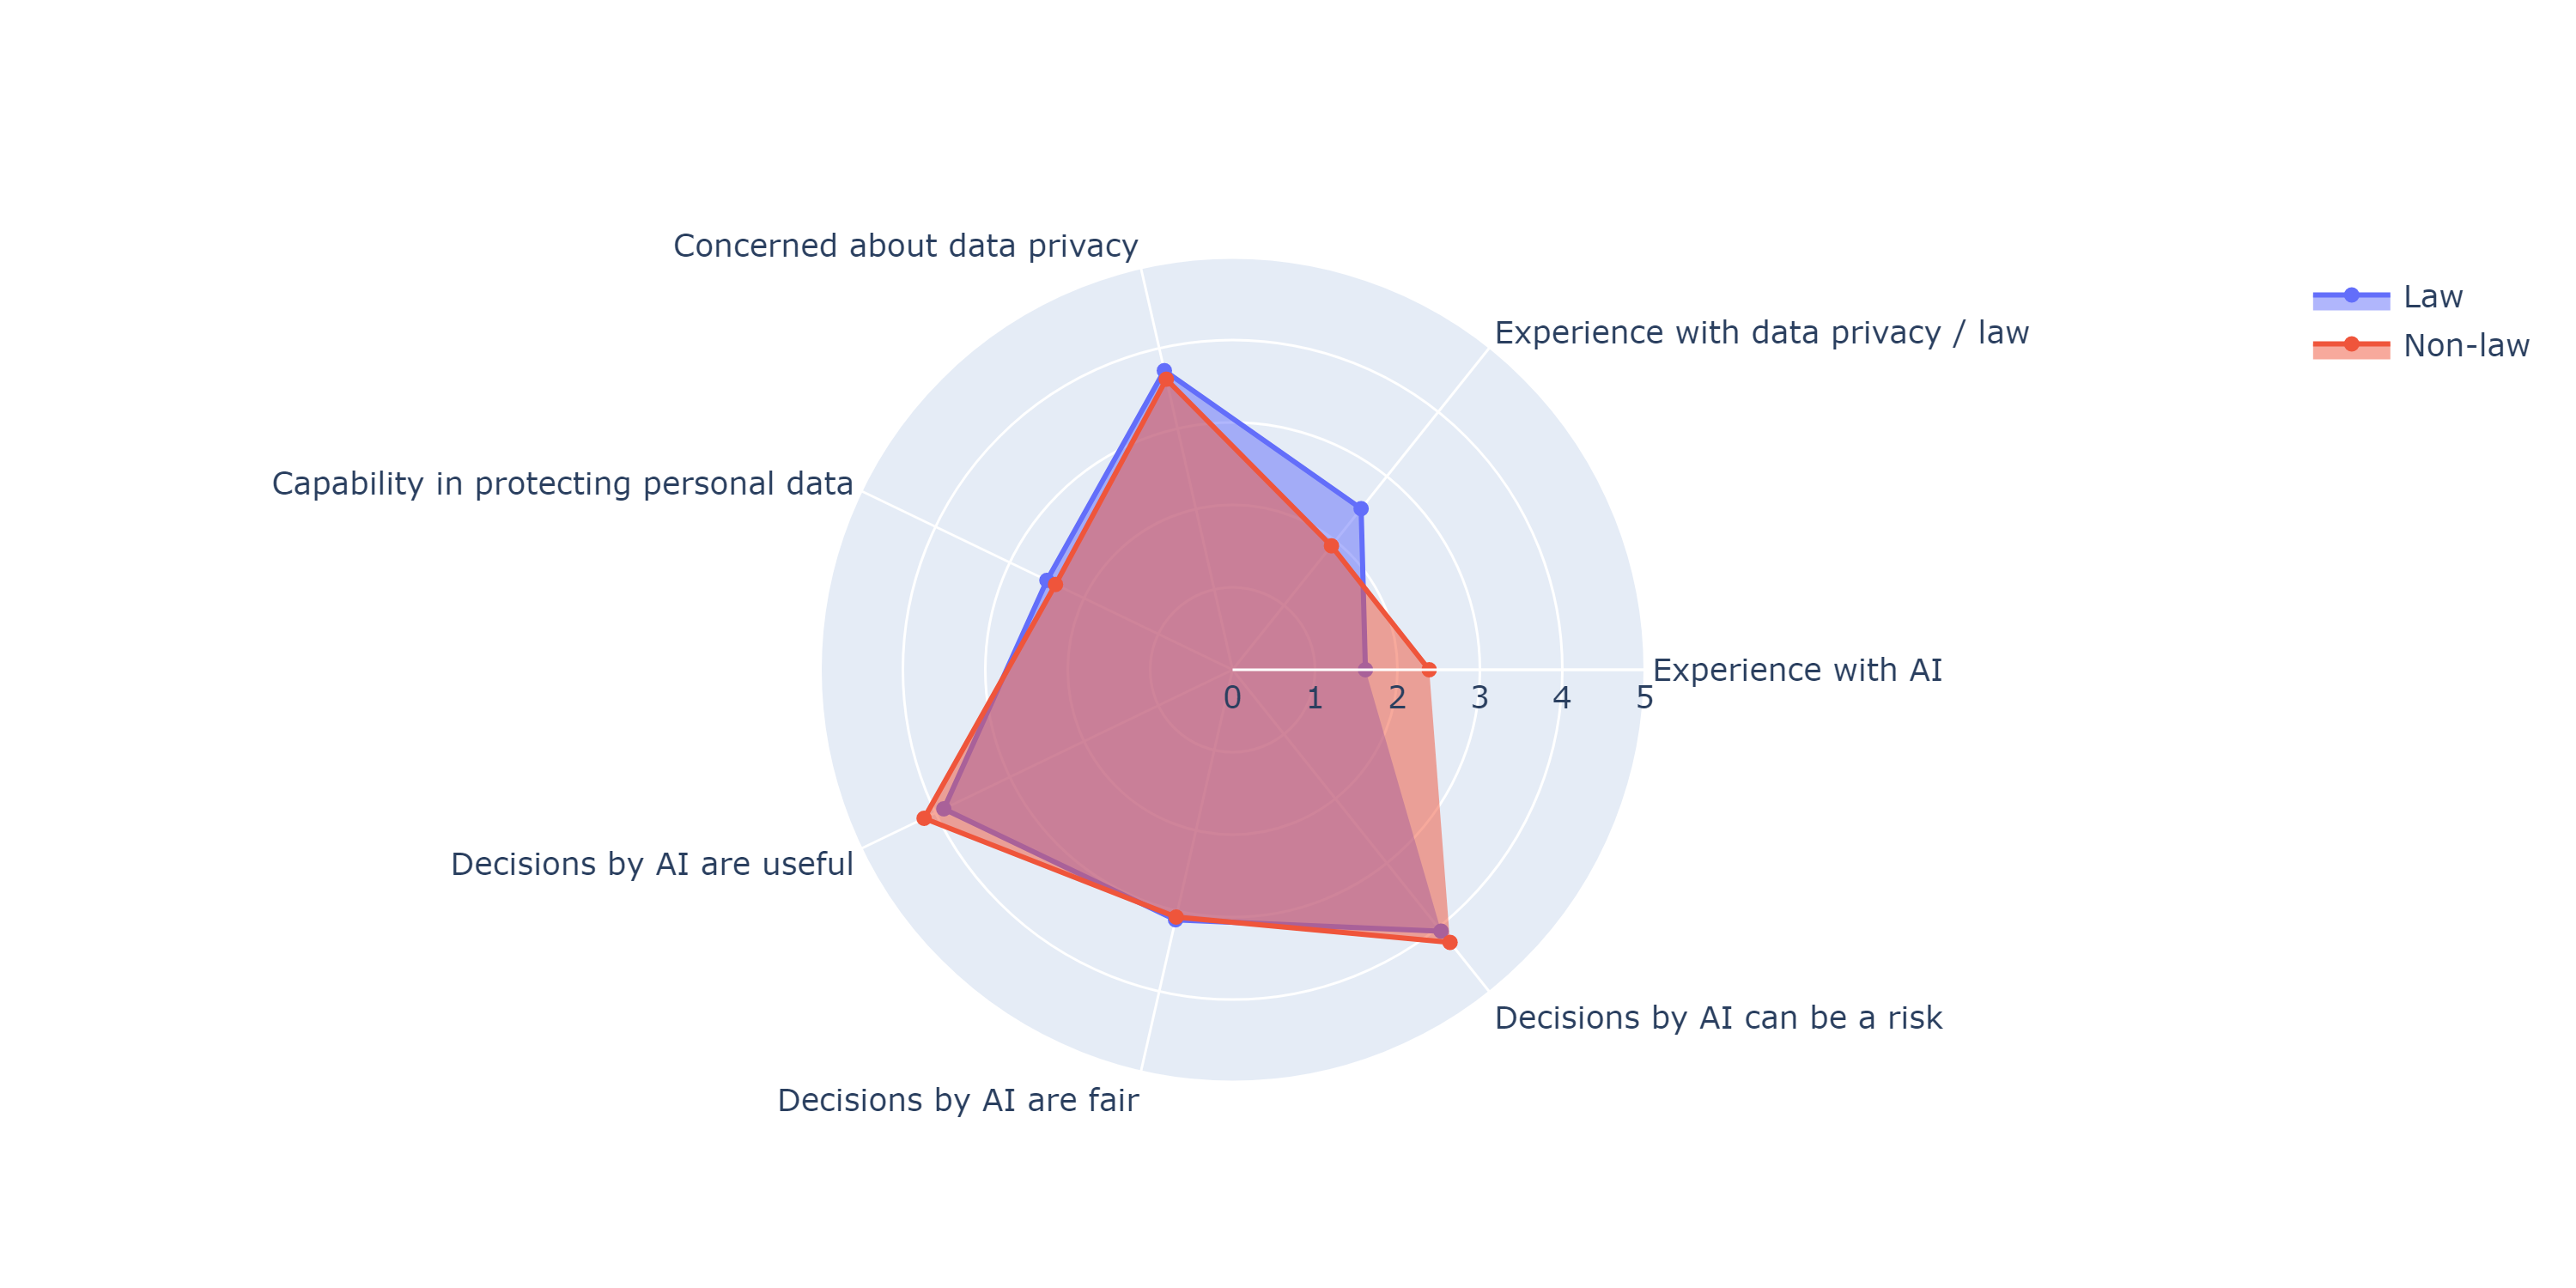
\includegraphics[width=1\linewidth]{figures/demo_3.png}
      \caption{Law vs Non-law respondents}
      %\label{fig:draketl}
    \end{subfigure}
    \hfill
    \begin{subfigure}[b]{1\textwidth}
      \centering
      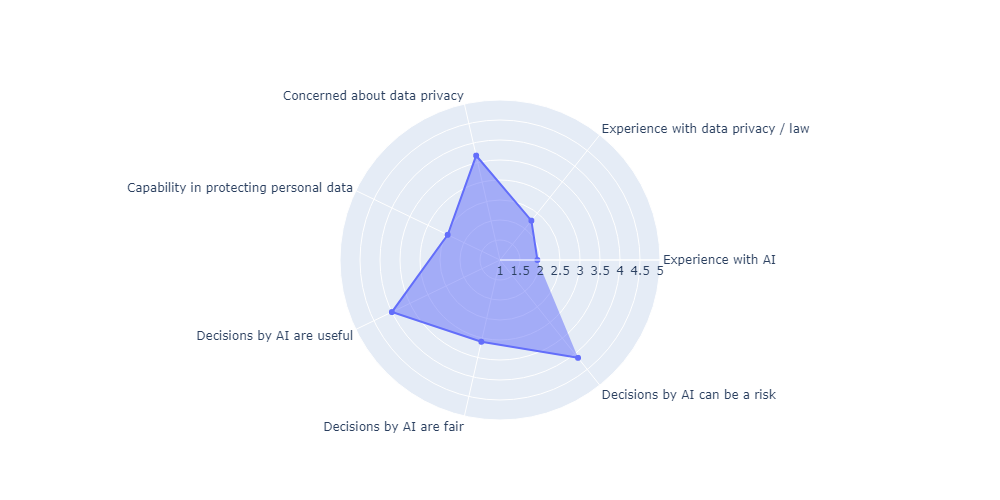
\includegraphics[width=1\linewidth]{figures/demo_4.png}
      \caption{All respondents}
    \end{subfigure}
    \caption{Mean scores of self-reported beliefs of respondents regarding AI \& data privacy. (1 = least agree, 5 = strongly agree. $n=31$)}
    \label{fig:demo_3}
\end{figure}

\subsection{Part 2 \& Part 6: Comparison of self-reported scores of explainability across the three contexts}
Using the Wilcoxon Rank Sum Test, I tested for the following, setting $\alpha = 0.1$: 
\begin{align*}
    H0&: \text{There is no increase / decrease in scores after viewing the explainations.} \\
    H1&: \text{There is an increase / decrease in scores after viewing the explainations.}
\end{align*}

The 1-sided test was used to check whether the distribution underlying the difference between the initial and final paired scores was symmetric below or above 0 (\cite{scipy}). Mathematically it can be stated as $d = i - f$, where $i$ and $f$ are the scores reported before and after viewing the explanations, and $d$ is the difference. Hence, if $d < 0$, then $i < f$ and the scores increased after viewing, and $d > 0$, then $i > f$ and the scores decreased after viewing.

\begin{table}[!ht]
    \centering
    \resizebox{\textwidth}{!}{    
    \begin{tabular}{|p{0.3\textwidth}|p{0.15\textwidth}|p{0.15\textwidth}|p{0.15\textwidth}|p{0.15\textwidth}|p{0.15\textwidth}|p{0.15\textwidth}|}
    \hline
        \textbf{Question} & \textbf{Context 1: Increase} & \textbf{Context 1: Decrease} & \textbf{Context 2: Increase} & \textbf{Context 2: Decrease} & \textbf{Context 3: Increase} & \textbf{Context 3: Decrease} \\ \hline
        \textbf{Do you think model is effective?} & \cellcolor{red!25}0.013 & 0.987 & 0.932 & \cellcolor{red!25}0.0684 & 0.856 & 0.144 \\ \hline
        \textbf{Do you think model is a fair method?} & 0.382 & 0.618 & 0.841 & 0.159 & 0.933 & \cellcolor{red!25}0.0671 \\ \hline
        \textbf{Do you think model is a risk to society?} & 0.756 & 0.244 & 0.428 & 0.572 & 0.825 & 0.175 \\ \hline
        \textbf{Do you trust the prediction of the model?} & 0.887 & 0.113 & 0.945 & \cellcolor{red!25}0.055 & 0.837 & 0.163 \\ \hline
    \end{tabular}
    }
    \caption{p-values comparing whether there was a statistically significant increase / decrease in the explainability scores before and after viewing explanations.}
    \label{tab:context_comparison}
\end{table}

\begin{table}[!ht]
    \centering
    \begin{subtable}{0.5\textwidth}
        \begin{tabular}{|l|l|}
        \hline
            \textbf{Context} & \textbf{p-value} \\ \hline
            1: Increase & 0.369 \\ \hline
            1: Decrease & 0.633 \\ \hline
            2: Increase & 0.940 \\ \hline
            2: Decrease & \cellcolor{red!25}0.060 \\ \hline
            3: Increase & 0.955 \\ \hline
            3: Decrease & \cellcolor{red!25}0.0450 \\ \hline
        \end{tabular}
        \caption{p-values averaged across metrics, compared by contexts}
        \label{tab:context_comparison_2a}
    \end{subtable}
    \hfill
    \begin{subtable}{0.5\textwidth}
        \begin{tabular}{|l|l|}
            \textbf{Metric}                                    & \textbf{p-value}                     \\ \hline
            Effective: Increase & 0.485  \\ \hline
            Effective: Decrease & 0.515  \\ \hline
            Fair: Increase      & 0.826  \\ \hline
            Fair: Decrease      & 0.174  \\ \hline
            Risk: Increase      & 0.660  \\ \hline
            Risk : Decrease     & 0.340  \\ \hline
            Trust: Increase     & 0.953  \\ \hline
            Trust: Decrease     & \cellcolor{red!25}0.0468 \\ \hline
        \end{tabular}
        \caption{p-values averaged across contexts, compared by metrics}
        \label{tab:context_comparison_2b}
    \end{subtable}
    \caption{p-values comparing aggregated scores by context and metric}
    \label{tab:context_comparison_2}
\end{table}

\begin{table}[!ht]
    \centering
    \begin{tabular}{|l|l|}
        \hline
        \textbf{Increase} & \textbf{Decrease} \\ \hline
        0.844             & 0.156           \\ \hline
    \end{tabular}
    \caption{p-values comparing aggregated scores across contexts and metrics}
    \label{tab:context_comparison_3}
\end{table}

The p-values are reported in Table~\ref{tab:context_comparison} ,~\ref{tab:context_comparison_2} and~\ref{tab:context_comparison_3}. "Increase" and "decrease" refer to the p-values of the test to check whether the scores significantly increased or decreased. Here are the instances when $p<0.1$, and therefore $H0$ can be rejected in favour of $H1$ such that there was a significant increase / decrease of scores after viewing the explanations:
\begin{enumerate}
    \item There is a statistically significant decrease in explainability for context 1 and 2 when aggregating across the metrics (Table~\ref{tab:context_comparison_2a}) and for trust when aggregating across the three contexts (Table~\ref{tab:context_comparison_2b}).
    \item In particular, effectiveness and trust significantly decreased for context 2, and fairness significantly decreased for context 3 (Table~\ref{tab:context_comparison}). 
    The overall explainability aggregated across both contexts and metrics did not significantly increase / decrease (Table~\ref{tab:context_comparison_3}).
\end{enumerate}

Here are some inferences that could be drawn from these observations:
\begin{enumerate}
    \item 
\end{enumerate}

\subsection{Part 3: Testing whether viewing more visualisations increase explainability}
From Figure~\ref{fig:part3_trend}, a decreasing trend of both understand and interpret after viewing each explanation, though understanding has a more negative gradient than interpret. Keeping in mind that the question asked was whether the respondent found the model's prediction more understandable and whether the visualisation was easier to interpret, respondents found the model less generally explainable after viewing more explanations, both in terms of the method of visualising the explanation, as well as understanding the inner logic of the model. 

A direct interpretation of this decreasing trend suggests that the model and LIME were not very effective. However, this could also be interpreted as the respondents being more confused about how the model works globally after being exposed to more nuanced details about the model, rather than being confused about a specific prediction of the model. As mentioned in Chapter~\ref{chapter2}, the visualisations for this part were specifically chosen to demonstrate the limits of the model by changing keywords which were strong predictors of the data practice. This means that respondents were getting a more complex (and confusing) conception of the model globally as they found contradictions in how the model used certain keywords in some examples but not in others. Therefore, each explanation was actually effective in communicating to the respondents how that particular prediction was made, but as a whole how the model functioned was not understandable given the contradictions between each explanation. This decrease in explainability could be likened to a variation of the Dunning-Kruger effect (\cite{dunning_kruger}), whereby the respondents who initially had no experience with the model believed that they understood the model well because they were unaware of the complexity of the model, but when they were given more information, they had more awareness of the complexity and therefore reported a drop in explainability of the model as a whole.

\begin{figure}[!ht]
    \centering
    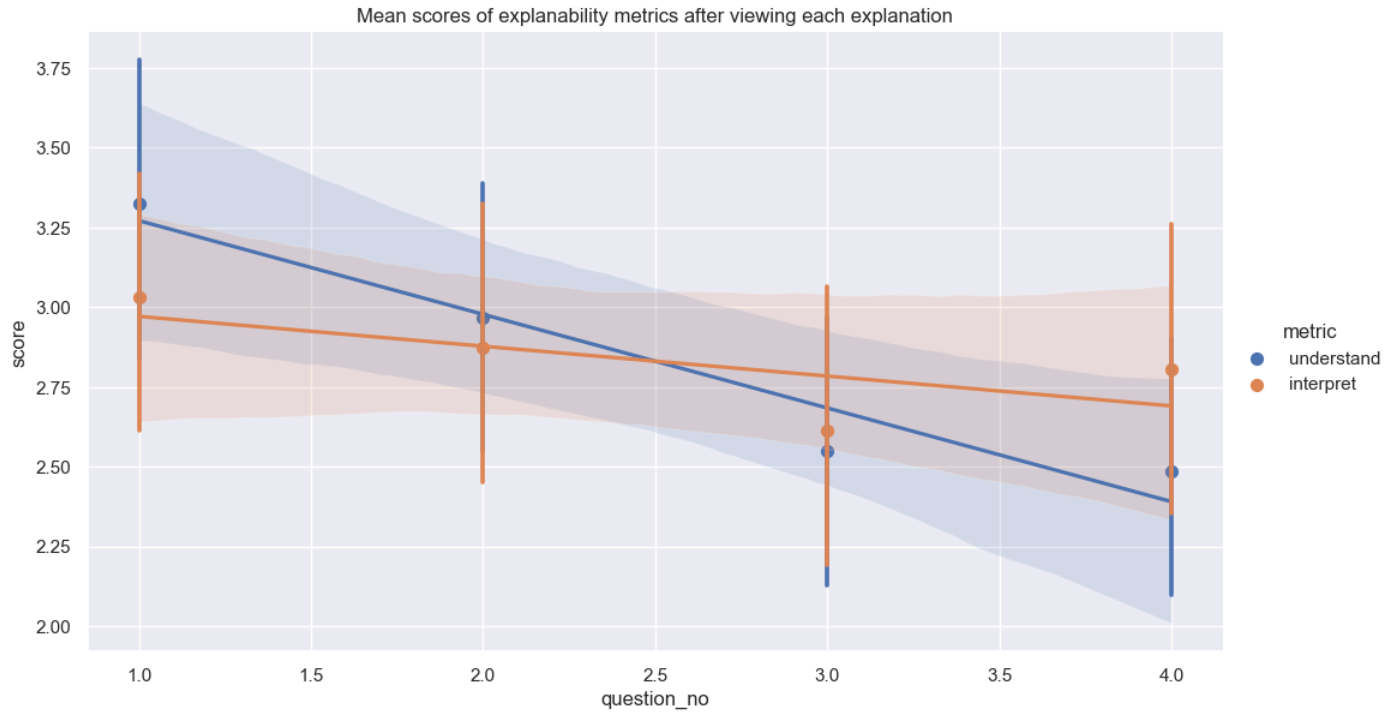
\includegraphics[width=1\linewidth]{figures/part3.png}
    \caption{Trend of the mean of self-reported understanding and interpretability after viewing each explanation}
    \label{fig:part3_trend}
\end{figure}

(need to add the visualisations for the counterfactuals here)

Since the model itself gave quite ambivalent predicted probabilities for each data practice, the respondents' votes of predicting whether these counterfactuals would be classified as \texttt{Identifier\_Cookie} should also be equally ambivalent if the respondents actually had a good sense of how the model would predict. Only the results of the first question had some similarity to the predicted probabilities of the model, while the results of the third question differed the most from the model. Nevertheless, given the lack of any consistent trend across the questions, it is difficult to draw any definitive interpretations from this section.

\begin{figure}[!ht]
    \centering
    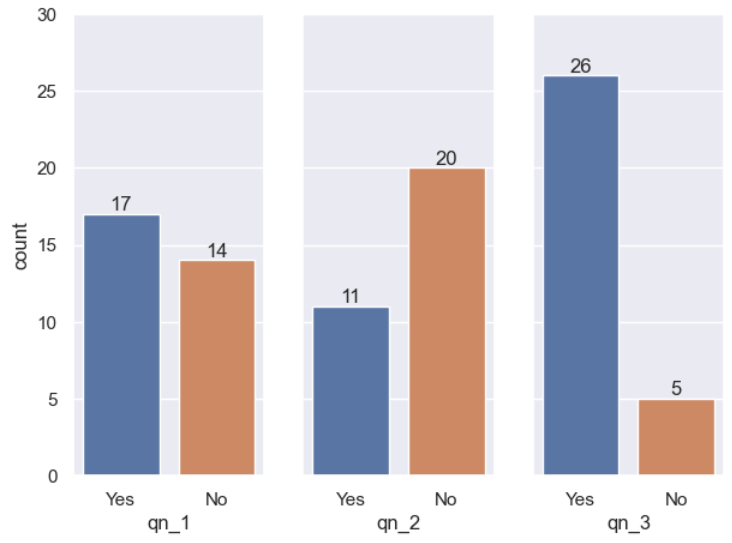
\includegraphics[width=1\linewidth]{figures/part_3_counterfactual.png}
    \caption{Votes for predicting whether counterfactual would be classified as \texttt{Identifier\_Cookie\_or\_Similar\_Tech\_1st\_Party}}
    \label{fig:part3_counterfactual}
\end{figure}

\subsection{Part 4 \& 5: Testing which model and word representation is more explainable}
Overall, respondents found no difference between logistic regression and SVC (Figure~\ref{fig:part4}), while it was more contentious for the word representation, with a third split across the three categories (Figure~\ref{fig:part5}). For logistic regression vs SVC, the results coincided with the performance of the classifiers. However for word representations , I found GloVE more explainable than Tf-IDF. While there is no majority consensus in favour of GloVe, the fact that the votes were almost equally split instead of being heavily weighted in favour of one category shows that respondents were more undecided. This means that while respondents might not be able to accurately discern which was the more explainable word representation as compared to an expert in the field, they still have some level of intuition when there are differences in the components of the models used. This suggests that LIME used in this context has a decent level of explainability, if not the distribution of votes for Part 4 \& Part 5 would be roughly equivalent.

\begin{figure}[!ht]
    \begin{subfigure}[b]{0.75\textwidth}
      \centering
      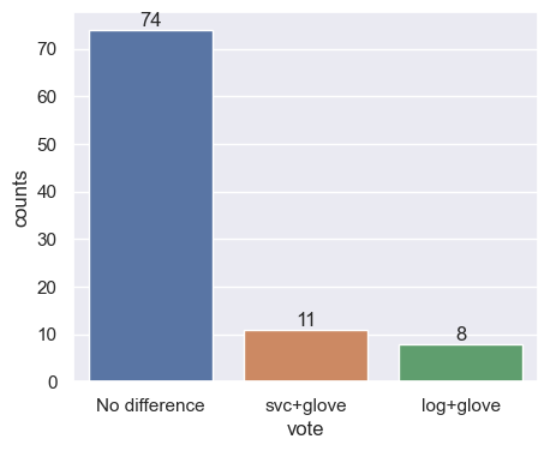
\includegraphics[width=1\linewidth]{figures/part4_votes.png}
      \caption{Total votes across 3 questions}
      %\label{fig:draketl}
    \end{subfigure}
    \hfill
    \begin{subfigure}[b]{1\textwidth}
      \centering
      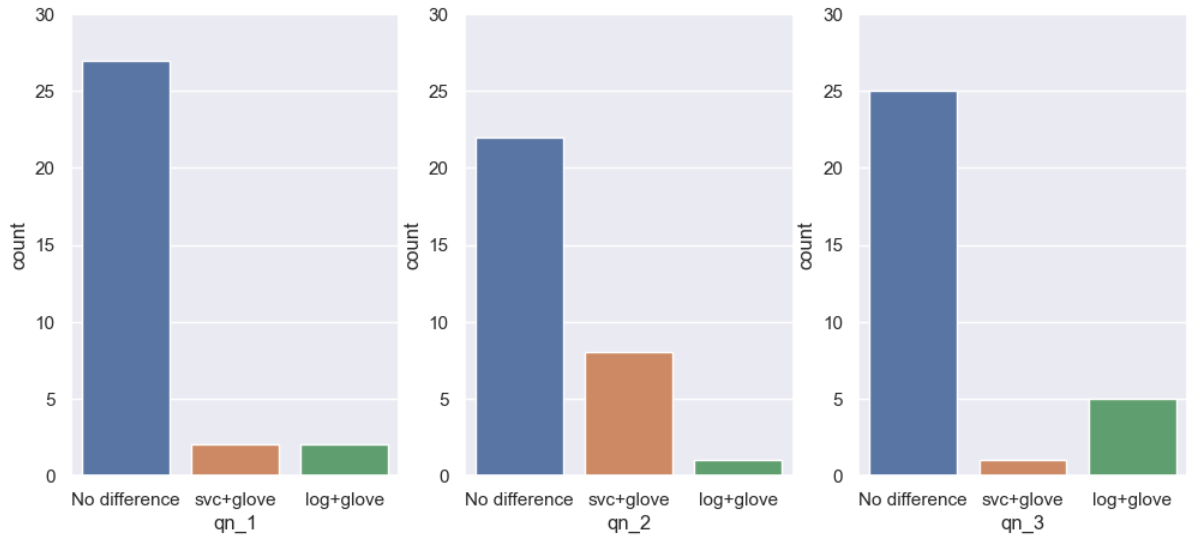
\includegraphics[width=1\linewidth]{figures/part_4_votes_1.png}
      \caption{Votes per question}
    \end{subfigure}
    \caption{Testing for which model was more explainable: Respondents' votes to whether SVC + GloVe or Logistic regression + GloVe were more explaninable}
    \label{fig:part4}
\end{figure}

\begin{figure}[!ht]
    \begin{subfigure}[b]{0.75\textwidth}
      \centering
      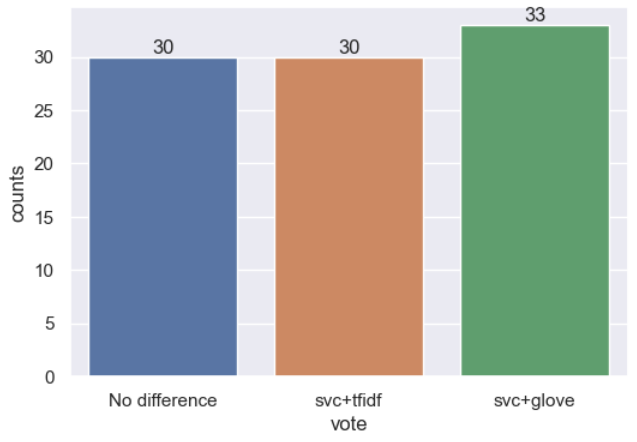
\includegraphics[width=1\linewidth]{figures/part5_votes.png}
      \caption{Total votes across 3 questions}
      %\label{fig:draketl}
    \end{subfigure}
    \hfill
    \begin{subfigure}[b]{1\textwidth}
      \centering
      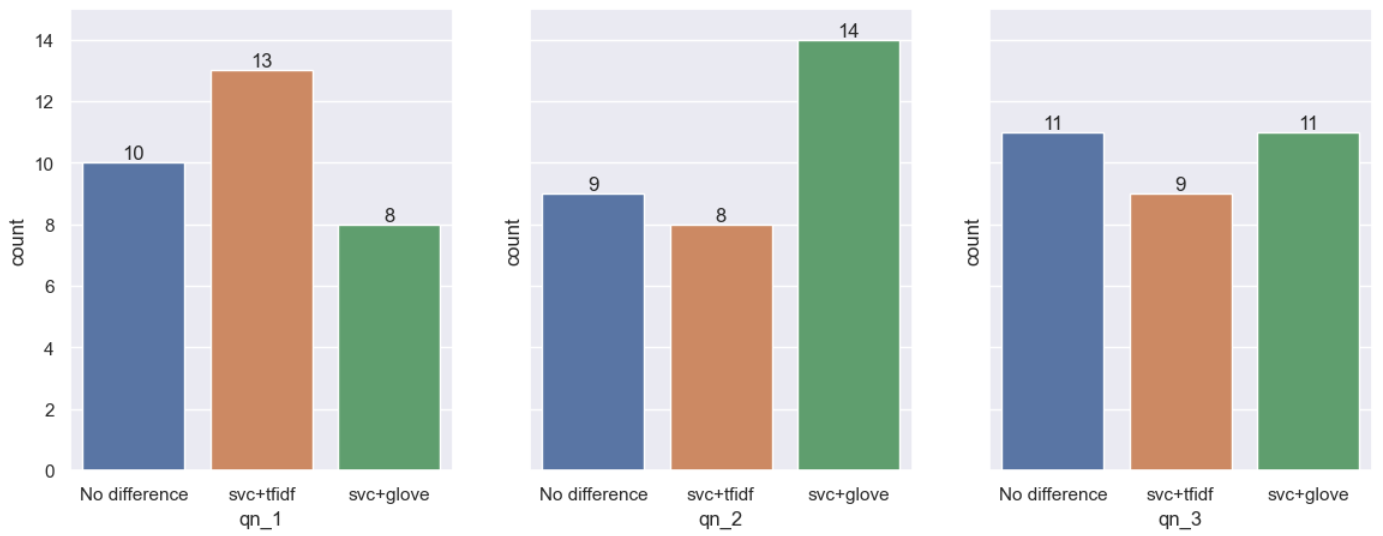
\includegraphics[width=1\linewidth]{figures/part_5_votes_1.png}
      \caption{Votes per question}
    \end{subfigure}
    \caption{Testing for which word representation was more explainable: Respondents' votes to whether SVC + TfIDF or SVC + GloVe were more explaninable}
    \label{fig:part5}
\end{figure}

\subsection{General interpretation of results}
